\documentclass{beamer}
\usepackage{graphicx}
\usetheme{default}
%\usecolortheme{seahorse}
\usepackage{default}
\usepackage{tikz}
\usetikzlibrary{shapes,arrows}

\setbeamertemplate{footline}[frame number]{}
\setbeamertemplate{navigation symbols}{}
\setbeamertemplate{frametitle}[default][center]
\setbeamerfont{frametitle}{shape=\scshape}


\usepackage{xcolor}
\usepackage{csquotes}
\usepackage{multirow}
\usepackage{media9}%
\newcommand{\includemovie}[3]{%
\includemedia[%
width=#1,height=#2,%
activate=pagevisible,%
deactivate=pageclose,%
addresource=#3,%
flashvars={%
src=#3 % same path as in addresource!
&autoPlay=true % default: false; if =true, automatically starts playback after activation (see option ?activation)?
&loop=true % if loop=true, media is played in a loop
&controlBarAutoHideTimeout=0 %  time span before auto-hide
}%
]{}{StrobeMediaPlayback.swf}}%


\newcommand{\col}[3]{
	\textcolor<#3->{red}{\textcolor<1-#2>{white}{#1}}
	}	

\newcommand{\colx}[3]{
	\textcolor<#3->{red}{\textcolor<1-#2>{black}{#1}}
	}



{\title{\textsc{Lecture 19: Bank Runs} \\ \tiny See Doepke, Lehnert, and Sellgren (1999) Ch. 17.4}
\author{Trevor Gallen}
\date{}

\begin{document}

\begin{frame}
\titlepage
\end{frame}

\begin{frame}
\frametitle{Introduction}
\begin{itemize}
\item<1-> We have a model of the macroeconomy
\bigskip
\item<2->  Includes intertemporal choice of consumption, labor, investment
\bigskip
\item<3->  Can deal with taxation, expenditure, transfers, money creation, bonds
\bigskip
\item<4->  Can discuss growth, business cycles, unemployment, interest rates, wages
\bigskip
\item<5->  There is no financial system...the closest we get is something like:
$$i=\frac{R}{P}-\delta$$
\item<6-> So we'll introduce a model of banks (and bank runs)
\end{itemize}
\end{frame}

\begin{frame}
\frametitle{The basic idea}
\begin{itemize}
\item<1-> Banks are going to do something good.  They'll:
\bigskip
\begin{itemize}
\item<2-> Take money (deposits)
\bigskip
\item<2-> Allow you to withdraw it at any time (liquidity)
\bigskip
\item<2-> Invest it for you and pay you for the right to loan it out (interest)
\bigskip
\end{itemize}
\item<3-> But there will be a big problem...what?
\bigskip
\item<4-> Because of how banks are structured, they'll be vulnerable to \textbf{bank runs}
\end{itemize}
\end{frame}

\begin{frame}
\frametitle{Diamond and Dybvig}
\begin{itemize}
\item<1-> Diamond and Dybvig:
\blockquote{Bank runs are a common feature of the extreme crises that have played a prominent role in monetary history. During a bank run, depositors rush to withdraw their deposits because they expect the bank to fail. In fact, the sudden withdrawals can force the bank to liquidate many of its assets at a loss and to fail. In a panic with many bank failures, there is a disruption of the monetary system and a reduction in production.}
\item<2-> The point: there are multiple equilibria.  If everyone thinks the bank will fail, it fails.  If people don't think it is fine, it will be.
\bigskip
\item<3-> We'll tell a highly stylized story about turnips now.  
\end{itemize}
\end{frame}

\begin{frame}
\frametitle{Key To Bank Runs and Financial Crises???}
\begin{figure}
\centering

\includegraphics[scale=0.05]{turnip.jpg}
\end{figure}
\end{frame}

\begin{frame}
\frametitle{Key To Bank Runs and Financial Crises???}
\begin{figure}
\centering

\includegraphics[scale=0.2]{turnip.jpg}
\end{figure}
\end{frame}

\begin{frame}
\frametitle{Key To Bank Runs and Financial Crises???}
\begin{figure}
\centering

\includegraphics[scale=0.85]{turnip.jpg}
\end{figure}
\end{frame}

\begin{frame}
\frametitle{A whole new world}
\begin{enumerate}
\item<1-> Our world starts off with a turnip technology: everything is turnips
\bigskip
\item<2-> Everyone starts off in period 0 with a turnip
\bigskip
\item<3-> They can all plant it (or give it to the bank to plant)
\bigskip
\item<4-> At the beginning of period 1, some proportion of the population $\theta$ finds out they'll die at the end of the period
\bigskip
\item<5-> Everyone can uproot their turnip and get 1 turnip back
\bigskip
\item<6-> At the beginning of period 2, all the turnips that are left grow to be $F>1$ turnips
\bigskip
\item<7-> If you're still alive, you can eat your turnip
\end{enumerate}
\end{frame}

\begin{frame}
\frametitle{Preferences}
\begin{itemize}
\item<1-> In this world everyone is perfectly patient (if alive).  Let:
\smallskip
\begin{itemize}
\item<2-> $c_1$ be consumption in period 1 
\smallskip
\item<2->  $c_2$ be consumption in period 2 
\smallskip
\item<3->  $\Theta$ be your ``type"
\smallskip
\begin{itemize}
\item<3->  $\Theta=1$ if you die in period 1
\smallskip
\item<3-> $\Theta=2$ if you die in period 2 
\end{itemize}
\end{itemize}
\item[]<4->  \ 
$$U(c_1,c_2,\Theta)=\left\{\begin{array}{ll}\log(c_1) & \text{if }\Theta=1 \\ Q\log(c_1+c_2) & \text{if }\Theta=2\end{array}\right\}$$
\item<4-> Where $1>Q>F^{-1}$, which will control how important it is to consume if you're the second type.
\item<5-> The point of these preferences is just to say:
\smallskip
\begin{itemize} 
\item<6-> ``People are have diminishing returns to consumption/are risk averse" 
\smallskip
\item<7->  ``The second type is willing to wait if it gains her anything"
\end{itemize}
\end{itemize}
\end{frame}

\begin{frame}
\frametitle{On your own}
\begin{itemize}
\item<1-> Imagine you're on your own in this world: what do you do?
\bigskip
\begin{enumerate}
\item<2-> Plant turnip in period 0
\bigskip
\item<3-> Enter period 1, find out type
\bigskip
\item<4-> If type 1 (die in period 1) then dig up turnip, eat 1 turnip, get $\log(1)$
\bigskip
\item<5-> If type 2 (die in period 2) then wait until period 2, dig up turnip, eat $F>1$ turnips, get $\log(F)$
\end{enumerate}
\item<7-> To put meat and bones on this, I'm going to say that $F=1.1$, and $\theta=0.5$, $1>Q>F^{-1}$ is, 0.98:
\bigskip
\item<8-> Then with probability $\theta$ you get utility $\log(1)=0$ and with probability $(1-\theta)$ you get utility $\log(1.1)=0.095$.  
\bigskip
\item<9-> On your own, you get expected utility:
$$\theta\cdot \log(1)+(1-\theta)\cdot\log(1.1)=0.5\cdot0+0.98 +0.5\cdot 0.095=0.046702$$
\end{itemize}
\end{frame}

\begin{frame}
\frametitle{Join together}
\begin{itemize}
\item<1-> Question:  can banks improve on this?  Can we gain by joining together?
\bigskip
\item<2-> Yes!  This is what insurance markets are for!
\bigskip
\item<3-> We could all pay a premium (give up our turnips) in period zero
\bigskip
\item<4-> If we find out we're type 1, insurance company digs up our turnip and a little of someone else's, pays us some amount greater than 1
\bigskip
\item<5-> If we find out we're type 2, insurance company will have some turnips left over, pays us some amount less than $F$ and greater than 1
\bigskip
\item<6-> We can all be better off by using insurance to smooth our consumption across states of the world
\end{itemize}
\end{frame}

\begin{frame}
\frametitle{Budget constraint of the insurance company}
\begin{itemize}
\item<1-> The insurance company will pay out $c_1^1$ to all individuals of type $1$ and $c_2^2$ to all individuals of type 2
\bigskip
\item<2-> Their budget constraint is, normalizing the population to 1,
$$\theta c_1^1 + \frac{(1-\theta)c_2^2}{F}=1$$
\bigskip
\item<3-> This is saying that I have 1 turnip: if I increase $c_1^1$ a little, I lose that whole amount (times the population weight).  If I increase $c_2^2$, I only have to leave $\frac{1}{F}$ turnips in the ground (times their population weight) in order to pay them.
\bigskip
\item<4-> If we wanted to graph to make the tradeoff clear, writing $c_1^1$ as a function of $c_2^2$, we get: 
$$c_1^1=\frac{1}{\theta}\left(1- \frac{(1-\theta)c_2^2}{F}\right)$$
\item<5-> Let's graph this, with $F=1.1$ and $\theta=0.5$
\end{itemize}
\end{frame}

\begin{frame}
\frametitle{Budget constraint example}
\begin{figure}
\centering
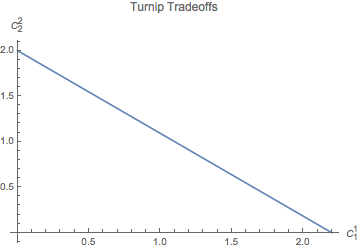
\includegraphics[scale=0.5]{turniptradeoff.png}
\end{figure}
\begin{itemize}
\item<2-> If you uproot the whole turnip and give it all to the half of the population that's type 1 in period 1, then they get 2 turnips each.
\smallskip 
\item<3-> If you uproot the whole $1.1$ turnip and give it all to the half of the population that's type 2 in period 2, then they get 2.2 turnips each.
\smallskip
\item<4-> Or you could do something in the middle
\end{itemize}
\end{frame}

\begin{frame}
\frametitle{Competition}
\begin{itemize}
\item<1->  What should the bank do?  Who should it pay?  Should it keep all the money?
\bigskip
\item<2-> If you don't do something that makes people as happy as possible, then another company will
\bigskip
\item<3-> Competition forces you to make the best decision for your population
\bigskip
\item<4-> Let's write down the utility maximization problem
\end{itemize}
\end{frame}

\begin{frame}
\frametitle{Insurance utility maximization}
$$\mathcal{L}(c_1^1,c_2^2,\lambda)=\theta \log(c_1^1)+(1-\theta)Q\log(c_2^2)+\lambda\left(1-\theta c_1^1-\frac{(1-\theta)c_2^2}{F}\right)$$
\begin{itemize}
\item Taking first order conditions, we get:
$$\begin{array}{lrcl}
\frac{\partial \mathcal{L}}{\partial c_1^1}: & \frac{\theta}{c_1^1}-\lambda\theta & = & 0 \\
\ \\
\frac{\partial \mathcal{L}}{\partial c_2^2}: & Q\frac{1-\theta}{c_2^2}-\lambda\frac{1-\theta}{F} & = & 0 \\
\ \\
\frac{\partial \mathcal{L}}{\partial \lambda}: & \theta c_1^1 + \frac{(1-\theta)c_2^2}{F}  & = & 1 \\
\end{array}$$
\bigskip
\item It's easy to solve these three equations for our three unknowns, $c_1^1$, $c_2^2$, and $\lambda$
\end{itemize}
\end{frame}

\begin{frame}
\frametitle{Insurance utility solution}
\begin{itemize}
\item Solving for $c_1^1$, $c_2^2$, and $\lambda$, we get:
$$c_1^1=\frac{1}{\theta+Q(1-\theta)}\ \ \ \ \ \ \ \ \ \ c_2^2=\frac{QF}{\theta+Q(1-\theta)}$$
\item<2-> Assuming that $1>Q>F^{-1}$ is, say, 0.98:
$$c_1^1=\frac{1}{0.5+0.98(1-0.5)}=1.\overline{01}$$
$$c_2^2=\frac{0.98\cdot 1.1}{\theta+0.98(1-\theta)}=1.0\overline{888}$$
\item<3-> Are people really better off?? They lose 0.011111 units if they're type 2 but only gain 0.010101 if they're type 1!
\item<4-> Recall we have to beat expected utility of 0.046702...let's see the expected utility
$$E_0(U(c_1^1,c_2^2,\Theta))=0.5\log(1.\overline{01})+0.5\log(1.0\overline{8})=0.046752$$
\item<5-> We did it!  Improved utility slightly.
\end{itemize}
\end{frame}

\begin{frame}
\frametitle{Insurance?}
\begin{figure}
\centering
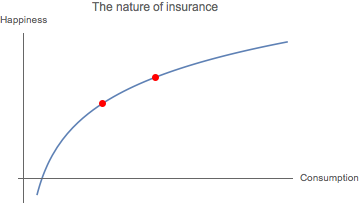
\includegraphics[scale=0.8]{Insurance_1.png}
\end{figure}
\end{frame}

\begin{frame}
\frametitle{Insurance?}
\begin{figure}
\centering
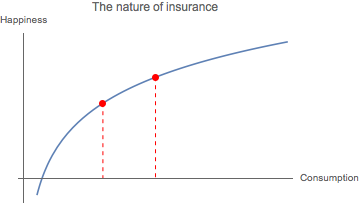
\includegraphics[scale=0.8]{Insurance_2.png}
\end{figure}
\end{frame}

\begin{frame}
\frametitle{Insurance?}
\begin{figure}
\centering
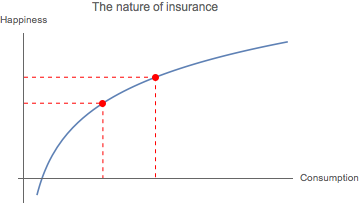
\includegraphics[scale=0.8]{Insurance_3.png}
\end{figure}
\end{frame}

\begin{frame}
\frametitle{Insurance?}
\begin{figure}
\centering
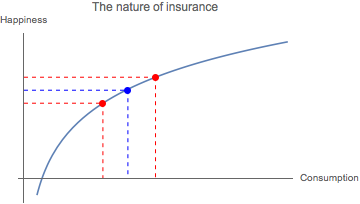
\includegraphics[scale=0.8]{Insurance_4.png}
\end{figure}
\end{frame}

\begin{frame}
\frametitle{Insurance?}
\begin{figure}
\centering
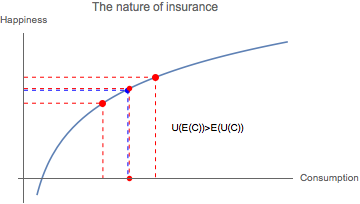
\includegraphics[scale=0.8]{Insurance_5.png}
\end{figure}
Utility of expected consumption preferred to expectation of utility.
\end{frame}


\begin{frame}
\frametitle{Insurance problem: summary}
\begin{itemize}
\item We have a problem in which people can invest and earn interest
\bigskip
\item But sometimes some people want their money now
\bigskip
\item Think of mortgages like planted turnips
\bigskip
\item Banks will allow people to withdraw whenever
\bigskip
\item People can benefit by participating in this ``insurance" system, where we're insuring your liquidity needs
\bigskip
\item Now we'll reframe this as a bank problem, but with one difference (what?)
\bigskip
\begin{itemize}
\item People can withdraw at any time! (No proof of type)
\end{itemize}
\end{itemize}
\end{frame}

\begin{frame}
\frametitle{Bank problem}
\begin{itemize}
\item Banks have the same problem as insurance companies, with a small twist:
\bigskip
\begin{enumerate}
\item They'll make promises in period 0 about how much you can receive if you withdraw in period 1 or period 2
\bigskip
\item They then have to keep those promises no matter how many people actually do withdraw in period 1
\end{enumerate}
\bigskip
\item The point:
\bigskip
\begin{itemize}
\item If too many people withdrew in period 1, then there would be nothing left in period 2!
\bigskip
\item If I fear too many people are going to withdraw in period 1, then I'll withdraw in period 1 even if I'm of type 2
\bigskip
\end{itemize}
\item Bank run!
\end{itemize}
\end{frame}

\begin{frame}
\frametitle{Bank problem}
\begin{itemize}
\item Banks face the same basic problem: choose an interest rate $r_1$ for type 1 and then whoever withdraws in period 2 gets the rest:
$$c_1^1=1+r_1$$
$$c_2^2=F\frac{1-\theta(1+r_1)}{1-\theta}$$
\item If for some reason $\theta$, the proportion that withdraw in period 1, is very high, then $c_2^2$ goes down.
\bigskip
\item If $c_2^2$ ever slips below $c_1^1$, then all the type 2's should run on the bank.
\bigskip
\item How should a bank choose $r_1$?
\bigskip
\item Maximize utility
\end{itemize}
\end{frame}

\begin{frame}
\frametitle{Bank maximization problem}
\begin{itemize}
\item Banks must maximize consumer expected utility, plugging in for $c_2^2$:
$$\theta\log(1+r_1)+(1-\theta)Q\log\left(F\frac{1-\theta(1+r)}{1-\theta}\right)$$
\item You can notice that this is the exact same problem as the insurance company faced, with $1+r_1=c_1$ and the budget constraint plugged in:
\bigskip
\item Consequently, it has the same maximization solutions: 
$$1+r_1=\frac{1}{\theta+Q(1-\theta)}$$
\item The bank chose the interest rate so everything is exactly the same as the insurance problem.
\bigskip
\item If all goes according to plan, type 1 will get $1.0\overline{1}$ and type 2 will get $1.0\overline{8}$
\bigskip
\item Type 2's won't want to run on the bank if nobody else is running on the bank, because they get more if they wait
\bigskip
\item But...
\end{itemize}
\end{frame}


\begin{frame}
\frametitle{Bank runs}
\begin{itemize}
\item What if for some reason I fear that too many people are withdrawing?  
\smallskip
\item Bank pays them out and I get the residual.  I should get $1.0\overline{8}$ if 50\% of population withdraws
\smallskip
\item What if 80\% withdraws?  Then I only get 
$$c_2^2=F\frac{1-\theta(1+r)}{1-\theta}=1.1\frac{1-0.6\cdot 1.0\overline{1}}{1-0.6}=1.05$$
\item Then I don't want to run
\smallskip
\item What if 89\% withdraws?  Then I get:
$$c_2^2=F\frac{1-\theta(1+r)}{1-\theta}=1.1\frac{1-0.89\cdot 1.0\overline{1}}{1-0.89}=1.001$$
\item If I fear that 89\% of the population should withdraw, then I'll withdraw too!
\smallskip
\item That means that (say) 90\% of the population is withdrawing, the heat is turned up for others who aren't withdrawing
\smallskip
\item Self-fulfilling Bank run!
\end{itemize}
\end{frame}

\begin{frame}
\frametitle{Bank runs: the story}
\begin{itemize}
\item If everyone is doing what they're supposed to, then there's no problem, everyone is happier and the economy is better than if there were no banks
\bigskip
\item But if I \emph{fear} too many people are withdrawing at once, then I should withdraw, creating a self-fulfilling bank run
\bigskip
\item This happens because banks make promises that they are able to keep only when people think they're able to keep them
\bigskip
\item Pro and con of banks:
\begin{itemize}
\item On the one hand, they improve utility
\bigskip
\item On the other hand, they're vulnerable to bank runs
\end{itemize}
\item Is there a way to avoid bank runs?
\end{itemize}
\end{frame}

\begin{frame}
\frametitle{Avoiding bank runs}
\begin{itemize}
\item There are a few possibilities to avoid bank runs (what?):
\bigskip
\begin{enumerate}
\item<2-> Suspension of convertibility
\bigskip
\item<3-> Deposit insurance
\bigskip
\item<4-> Mutual funds
\bigskip
\item<5->  Lender of last resort
\bigskip
\end{enumerate}
\item<5-> Let's talk about each in turn
\end{itemize}
\end{frame}

\begin{frame}
\frametitle{Suspension of convertibility}
\begin{itemize}
\item<1-> What is suspension of convertibility?
\bigskip
\item<2-> Government comes in and says: ``only $\theta$ of you will be able to withdraw today."  
\bigskip
\item<3-> Then as a type 2, I know I'm safe:  even if all the other type 2's try and succeed at withdrawing (which would be bad for the type 1's) then I will still get my due
\bigskip
\item<4-> Consequently, none of the type 2's will line up, and everything is wonderful
\bigskip
\item<5-> This method fails if you don't know $\theta$ in advance!  It would be a bad day for many of the type 1's if the government declared that only 25\% of the population can withdraw!
\end{itemize}
\end{frame}

\begin{frame}
\frametitle{Deposit insurance}
\begin{itemize}
\item<1-> What is deposit insurance?
\bigskip
\item<2-> Government comes in and says:  ``you don't need to withdraw: we'll insure your turnips"  
\bigskip
\item<3-> Then as a type 2, I know I'm safe:  even if all the other type 2's try and succeed at withdrawing I will still get my due
\bigskip
\item<4-> Consequently, none of the type 2's will line up, and everything is wonderful
\bigskip
\item<5-> This method can be expensive, because it insures both \emph{illiquid} and \emph{insolvent} banks!
\end{itemize}
\end{frame}

\begin{frame}
\frametitle{Mutual funds}
\begin{itemize}
\item<1-> What are mutual funds?
\bigskip
\item<2-> Banks don't make promises: they make investments and will return to you your liquidated value of the joint portfolio
\bigskip
\item<3-> For instance, if everyone is liquidating, then we only get 1 turnip each
\bigskip
\item<4-> As a type 2, I'm not scared that type 1's will take my money because the amount they're promised changes (they don't have a claim on my share)
\bigskip
\item<5-> This method works, unless you decide that mutual funds really have promised implicitly (which is what happened in the financial crisis to MMMF's)
\end{itemize}
\end{frame}

\begin{frame}
\frametitle{Lender of Last Resort}
\begin{itemize}
\item<1-> When under the threat of a bank run, there's one additional means of stopping it
\bigskip
\item<2-> Bank runs are a problem because banks are solvent, but illiquid
\bigskip
\item<3-> We can solve this problem by flooding the system with liquidity
\bigskip
\item<4-> Have Lender of Last Resort give cash loans in exchange for illiquid but good assets 
\bigskip
\item<5-> If we all want money, Federal Reserve can give banks cash and take good mortgages as collateral
\bigskip
\item<6-> The possibility that they'll do this makes a run not happen
\bigskip
\item<7-> This is called \textbf{Bagehot's Rule}: in times of crisis, lend without limit, to solvent firms, against good collateral, at high rates.
\end{itemize}
\end{frame}


\begin{frame}
\frametitle{Summing up}
\begin{itemize}
\item<1-> The history of finance is rife with bank runs
\smallskip
\item<2-> Fundamentally, it's a problem of multiple equilibria: fear of a run can create it.
\smallskip
\item<3-> We created the Federal Reserve to stop this! 
The Federal Reserve Act of 1913's official title was:\emph{``An Act To provide for the establishment of Federal reserve banks, to furnish an \textbf{elastic currency}, to afford means of \textbf{rediscounting commercial paper}, to establish a more effective supervision of banking in the United States, and for other purposes"}
\smallskip
\item<4-> Be a lender of last resort: be willing to make cash loans against those good but illiquid assets for cash
\smallskip
\item<5-> From 1818-1913, we had 9 financial crises, some very extreme (1 every $\sim$10 years)
\smallskip
\item<6-> After 1913, we've had 2 (1 every $\sim$ 50 years)
\smallskip
\item<7-> We know how to solve! Flood the system with liquidity.
\end{itemize}
\end{frame}

\end{document}



